\documentclass[french]{article}
\usepackage{geometry}
\geometry{a4paper}
\usepackage{graphicx}
\usepackage{amssymb}
\usepackage{amsmath}
\usepackage{amsthm}
\usepackage{empheq}
\usepackage{mdframed}
\usepackage{booktabs}
\usepackage{graphicx}
\usepackage{color}
\usepackage{psfrag}
\usepackage{pgfplots}
\usepackage{bm}
\usepackage[utf8]{inputenc}
\usepackage[T1]{fontenc}
\usepackage{babel}
\usepackage{indentfirst}
\usepackage{float}
\usepackage{enumitem}
\usepackage{subcaption}
\usepackage{hyperref}



\definecolor{ocre}{RGB}{243,102,25}
\definecolor{mygray}{RGB}{243,243,244}

\newcommand\orangebox[1]{\fcolorbox{ocre}{mygray}{\hspace{1em}#1\hspace{1em}}}

\newtheoremstyle{mytheoremstyle}
    {3pt}
    {3pt}
    {\normalfont}
    {0cm}
    {\rmfamily\bfseries}
    {.}
    {1em}
    {{\color{ocre}\thmname{#1}~\thmnumber{#2}}\thmnote{\,--\,#3}}
\newtheoremstyle{myproblemstyle}
    {3pt}
    {3pt}
    {\normalfont}
    {0cm}
    {\rmfamily\bfseries}
    {.}
    {1em}
    {{\color{black}\thmname{#1}~\thmnumber{#2}}\thmnote{\,--\,#3}}
\theoremstyle{mytheoremstyle}
\newmdtheoremenv[
    backgroundcolor=mygray,
    linecolor=ocre,
    leftmargin=0pt,
    innerleftmargin=20pt,
    innerrightmargin=20pt,
]{theorem}{Theorem}[section]
\theoremstyle{mytheoremstyle}
\newmdtheoremenv[
    backgroundcolor=mygray,
    linecolor=ocre,
    leftmargin=0pt,
    innerleftmargin=20pt,
    innerrightmargin=20pt,
]{definition}{Definition}[section]
\theoremstyle{myproblemstyle}
\newmdtheoremenv[
    linecolor=black,
    leftmargin=0pt,
    innerleftmargin=10pt,
    innerrightmargin=10pt,
]{problem}{Problem}[section]

\usepgfplotslibrary{colorbrewer}
\pgfplotsset{width=8cm,compat=1.9}

\title{Approches Deep Learning à la détection d'anomalies dans un système à temps réel}
\author{Mohamed-Amine ROMDHANE, Adam BOND\\Encadré par: Pr. Enrico Formenti}
\date{}

\begin{document}
    \maketitle

    \tableofcontents
    \clearpage

    \section{Introduction}
    Dans le cadre d'un besoin d'une startup spécialisée dans des services d'optimisation de consommation d'eau dans le milieu agricole, on veut pouvoir mettre en place un modèle de détection d'anomalies matérielles via les méthodes d'apprentissage automatique et de l'intelligence artificielle. Dans cette optique, cette entreprise a installé des senseurs sur des pompes à eaux qui en indiquant la pression à l'intérieur, permettent d'indiquer l'état d'irrigation. Celle-ci est déclenchée automatiquement à l'aide de capteurs d'humidité du sol.     
    \section{Problématique \& Hypothèses}
    Les senseurs de pression d'eau d'une pompe ne sont pas parfaits, et ils peuvent envoyer des valeurs légèrement différentes entre deux lectures. De plus, certains facteurs comme la chaleur ou l'humidité qui varient naturellement font en sorte que les courbes de ces senseurs ont toujours un bruit de basse amplitude. Il peut aussi arriver qu'une bulle d'air ou un petit objet passe temporairement par la pompe et devienne une "dent" sur le graphe de suivi de pression d'eau, c'est à dire une forte perturbation d'amplitude en un court moment.
    \newline
    \indent Le fonctionnement normal d'une pompe ressemble donc à une période calme perturbée uniquement par un bruit global, puis lorsque le capteur détecte que l'irrigation est nécessaire la courbe grimpe jusqu'à son maximum, et y reste jusqu'à ce que le capteur détecte que la terre est suffisamment irriguée. S'ensuit une chute brusque de la pression puis un retour au calme jusqu'au prochain cycle.
    \newline
    \indent Dans le cadre de cet étude, on a deux problèmes. Le premier est celui de la disponibilité des données. Le contact limité avec l'entreprise en ai une raison. Le second problème c'est que le modèle réel a beaucoup trop de variables, les senseurs dépendent les uns des autres et les bruits ainsi que les anomalies ont plusieurs sources et facteurs. 
    \newline
    \indent Le but de ce projet est au final de développer des approches d'apprentissage profond. Avec le peu de données qu'on a, la solution était de faire nos propres données qui s'approchent au mieux de ce qu'on nous a communiqué.
    \section{Les données}
    Faute de manque de données, nous nous sommes fixés la  création d'un outil permettant de générer des courbes d'états ressemblant à celles utilisés par l'entreprise. Cet outil devrait être modulaire pour permettre de simuler toutes les situations auxquelles l'entreprise est confrontée, incluant les anomalies. Il faut donc prévoir des paramètres permettant de varier le temps entre les cycles de pression, le nombre d'anomalies, leur type, le bruit, la fonction de transition entre états, etc...
        \subsection{Simulation des données}
        Le simulateur \textit{simulator.py} simule un système à temps réel. Ce dernier regroupe plusieurs variables dont:
        \begin{itemize}[label={•}]
            \item \textbf{realtime\_tick} l'écroulement temporel en millisecondes avant l'enregistrement d'un échantillon. Cette variable s'incrémente par \textit{dt\_per\_sample} après chaque échantillon.
            \item \textbf{dt\_per\_sample} c'est le temps en secondes entre chaque étape de simulation (temps entre deux échantillons).
            \item \textbf{transition\_type} est la fonction de transition entre états (exemple: East-In-Out Quad, Ease-In-Out Sine, Linear...). Pour conserver le nombres d'échantillons qu'on a, pour un état $A$ et $B$ où la différence d'amplitude est importante, on prend par exemple, les $n$ derniers échantillons de $A$ et et les $n$ premiers échantillons de $B$ et on applique la fonction de transition les $2n$ échantillons.
            \item \textbf{noise} est la fonction de bruit global présent dans le système (exemple: "gaussian" pour un bruit gaussien). Le bruit a son propre amplitude. 
            \item \textbf{states} est la liste d'états. Chaque état a une durée, une amplitude, et la liste (vide ou pas) des anomalies (appelées impulsions dans le contexte de simulation). Une \textit{anomalie} a sa propre durée, le temps de son début ainsi que son amplitude.
        \end{itemize}
        \subsection{Génération des données}
    \section{Deep Learning avec TensorFlow}
        \subsection{Approche naïve avec CNN}
        La première idée qu'on a eu était d'utiliser le réseau neuronal convolutif de TensorFlow (convolutional neural networks, abbrv: cnn) pour l'entraîner à reconnaître les images provenant d'un système stable ainsi qu'un système à forte perturbations admettant plusieurs anomalies. Vu que précédemment on a déjà généré 1000 images pour chacune de nos classes \textbf{stable} et \textbf{malfunction}, on les a alors importées pour être pré-traitées avant de les brancher au réseau. Dans le prétraitement, on redimensionne la taille de l'image (originalement 640x480) à 250x250. Vu que la couleur de l'image n'a pas d'importance, on redéfini sa gamme de couleur comme étant du \textit{grayscale}. Cette manipulation a le bénéfice d'avoir un tensor de dimension (250x250x1) au lieu de (250x250x3). On défini le nombre d'\textit{epochs} comme étant égale à 10 et le nombre de \textit{batchs} de données à être traité simultanément dans le réseau de neurones est égale à 10. Notre modèle TensorFlow a le pipeline décrit ci-dessous:
        \begin{center}
            Une \textbf{couche de convolution} à 2 dimensions avec \textbf{16} filtres, un noyau de taille \textbf{3x3} et la fonction de correction \textbf{RELu}. \\
            $
            \downarrow
            $\\
            Une \textbf{couche de pooling} où on prend que le \textbf{maximum} à l'issue des résultats précédents. \\
            $
            \downarrow
            $\\
            Une \textbf{couche de convolution} à 2 dimensions avec \textbf{32} filtres, un noyau de taille \textbf{3x3} et la fonction de correction \textbf{RELu}. \\
            $
            \downarrow
            $\\
            Une \textbf{couche de pooling} où on prend que le \textbf{maximum} à l'issue des résultats précédents. \\
            $
            \downarrow
            $\\
            Une \textbf{couche de convolution} à 2 dimensions avec \textbf{64} filtres, un noyau de taille \textbf{3x3} et la fonction de correction \textbf{RELu}.\\
            $
            \downarrow
            $\\
            Une \textbf{couche entièrement connectée} avec \textbf{512} neurones et une fonction d'activation \textbf{RELu}.\\
            $
            \downarrow
            $\\
            Une seul neurone avec la fonction d'activation \textbf{Sigmoïd}.
        \end{center}
        Avec 
        \[
        RELu(x) = \begin{cases}
            x,& \text{si } x \ge 0\\
            0,& \text{sinon}
        \end{cases}
        \]
        et
        \[
        Sigmoid(x) = \dfrac{1}{1+e^{-x}}
        \]
        \begin{figure}[H]
            \centering
            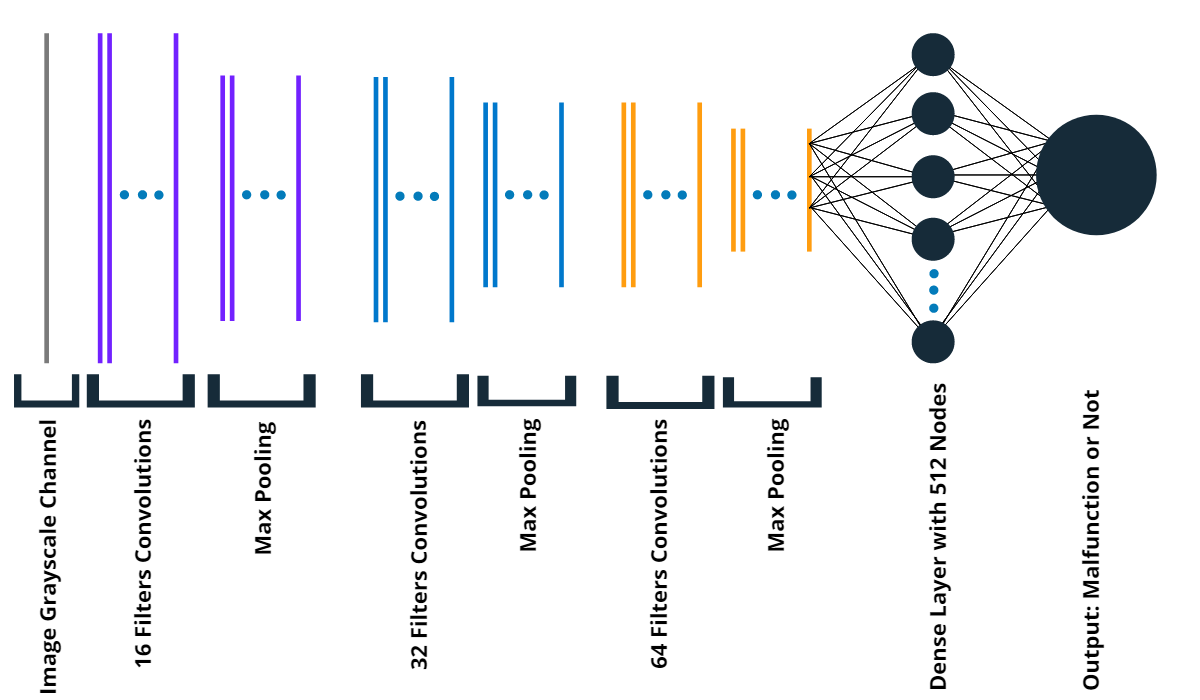
\includegraphics[width=\textwidth]{images/cnn.png}
            \caption{Le modèle CNN de classification d'anomalies}
            \label{}
        \end{figure}
        Notre modèle est compilé avec 2 ensembles d'images distincts. Un ensemble d'images d'entraînement et un ensemble de validation. En total, on a 2200 images pour l'entraînement et 2200 images pour la validation.
        \newline
        \begin{itemize}
            \item L'ensemble d'entraînement comporte 1100 images étiquetées \textbf{stable} ainsi que 1100 images étiquetées \textbf{malfunction}.
            \item L'ensemble de validation comporte le même nombre d'images pour chacune des deux classes mais des instances différentes de ceux dans l'ensemble l'entraînement.
        \end{itemize}
        Dans la section 5, on explique les résultats qu'on a eu suivant cette approche et pourquoi elle est naïve.
        \subsection{Extraction des features avec TSFresh}
        Afin d'accompagner nos méthodes de détection d'anomalies, nous avons cherché à trouver des approches permettant de détecter avec succès des anomalies sans devoir nourrir le modèle d'un ensemble de données conséquents, que ce soit des milliers de datapoint au format texte ou une image.
        Nous avons pour cela utilisé une libraire Python appelée TSFresh. TSFresh est un outil spécialement conçu pour analyser des séries temporelles en calculant un grand nombre de caractéristiques communes aux séries temporelles\cite{tsfreshfeatures}. La librairie cherche par exemple les coefficients de la série de fourier representée par le signal (fft\_coefficient), où bien le pourcentage de valeurs qui sont présente plus d'une fois, etc. Une fois ces features calculées, TSFresh utilise chacune des features individuellement en essayant de déterminer son efficacité pour prédire correctement la classification d'une série, et lui assigne une p-value en conséquence. En fonction de cette p-value, un algorithme statistique décide de qualifier cette feature comme pertinente ou non.
        
        \begin{figure}[H]
            \centering
            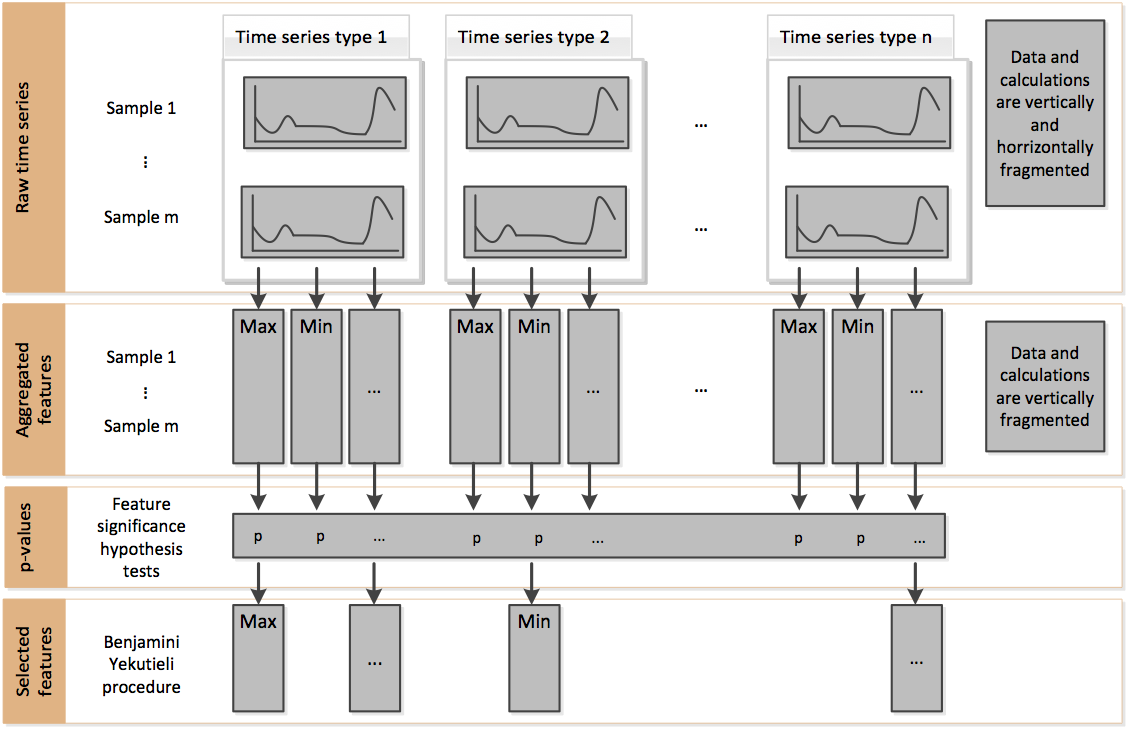
\includegraphics[width=.8\textwidth]{images/features_extraction.png}
            \caption{Image de la documentation TSFresh permettant de visualiser la sélection de features à partir des séries temporelles en entrée.}
            \label{}
        \end{figure}
        
        
        Nous avons d'abord tenté de réaliser cette analyse sur une matrice de pixels représentant l'image. Ainsi à chaque moment T équivaut une colonne de pixels blancs ou rouge, tous les pixels inférieurs à la valeur de l'amplitude étant coloriés en rouge et les autres laissés blancs. Nous avons rapidement abandonné cette idée puisqu'en plus de ne pas apporter plus d'informations par rapport à une simple série où équivaut à chaque moment T une valeur d'amplitude, elle apporte énormément d'informations superflues que TSFresh doit trier, et qui ralentissent le processus et rendent les résultats moins efficaces. Nous avons donc implémenté dans le simulateur un moyen d'exporter dans un fichier texte de nombreuses séries générées aléatoirement et identifiées selon si elles présentent des anomalies ou non.
        
        Une fois cela réalisé, nous avons donné les 1024 séries résultantes au logiciel pour calculer les coefficients. TSFresh a calculé plus de 800 features, dont il a considéré 305 commes pertinentes.
        
\begin{figure}[H]
            \centering
            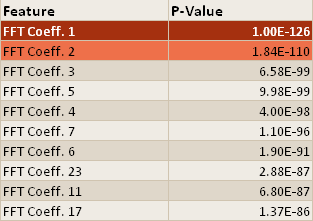
\includegraphics[width=0.35\textwidth]{images/features_pvalue.png}
            \caption{Table des P-Values des 10 features les plus significatives.}
            \label{}
        \end{figure}

        Parmi les 305 features, plus de la moitié étaient des coefficients d'une transformée de Fourier, et 48 parmi les 50 premières. Comme on peut le voir sur la table, les premières features et particulièrement la toute première, ont des P-Value extrêmement basses, un ordre de grandeur plus petites que les suivantes.
        
        Nous avons vérifié la pertinence de ces features en entraînant deux arbres de décision pour classer les séries temporelles en entrée dans deux classes : stable et malfonction.
        
        Nous avons donné au premier arbre de décision les données brutes, et il a obtenu une précision de 85\% sur les données de test. Nous avons donné aux second arbre uniquement les features extraites par TSFresh et la précision est montée à 90\%.
        
        Nous avons alors décidé de tester ces résultats en comparant la précision d'arbres de décisions qui prendraient uniquement en compte les N premières features afin d'essayer d'obtenir un ensemble de features aussi restreint que possible pouvant rendre la prédiction rapide. 
        
        Les résultats obtenus ont été que bien qu'une tendance se dégage à une plus grande précision plus on prend de features, la différence n'est pas énorme. On obtient 90\% de précision avec les 100 premières features (soit autant qu'avec les 305 features pertinentes), mais la précision est déja de 85\% avec uniquement la première feature, et de  89% avec les cinq premières.
        
        Afin de limiter l'overfit nous avons aussi vérifié et limité la profondeur maximum des arbres de décisions, mais nous nous sommes rendu compte qu'en réalité même avec toutes les features pertinentes, la profondeur de l'arbre ne dépassait jamais 18. C'est à dire que dans tous les cas, l'arbre de décision choisit d'utiliser un nombre restreint de features.
        
        Ces résultats confirment l'impact énorme des premiers features sélectionnés qui ont des P-Values étant plus petites d'un ordre de grandeur.
    
        \subsection{Détection d'anomalies en tant qu'objets}
        Dans le but de couvrir d'autres approches intéressantes, on s'est mit a chercher les techniques les plus récentes pour traiter les deux thèmes de ce travail de recherche: \textit{détection d'anomalies} et \textit{temps réel}. Une techniques qui nous a marqué le plus est celle de la détection d'objets. L'article Wikipédia \cite{odwikipedia} en anglais parle de ce sujet. On peut aussi voir dans la figure ci-dessous un exemple d'une telle détection d'objets réels.
        \begin{figure}[H]
            \centering
            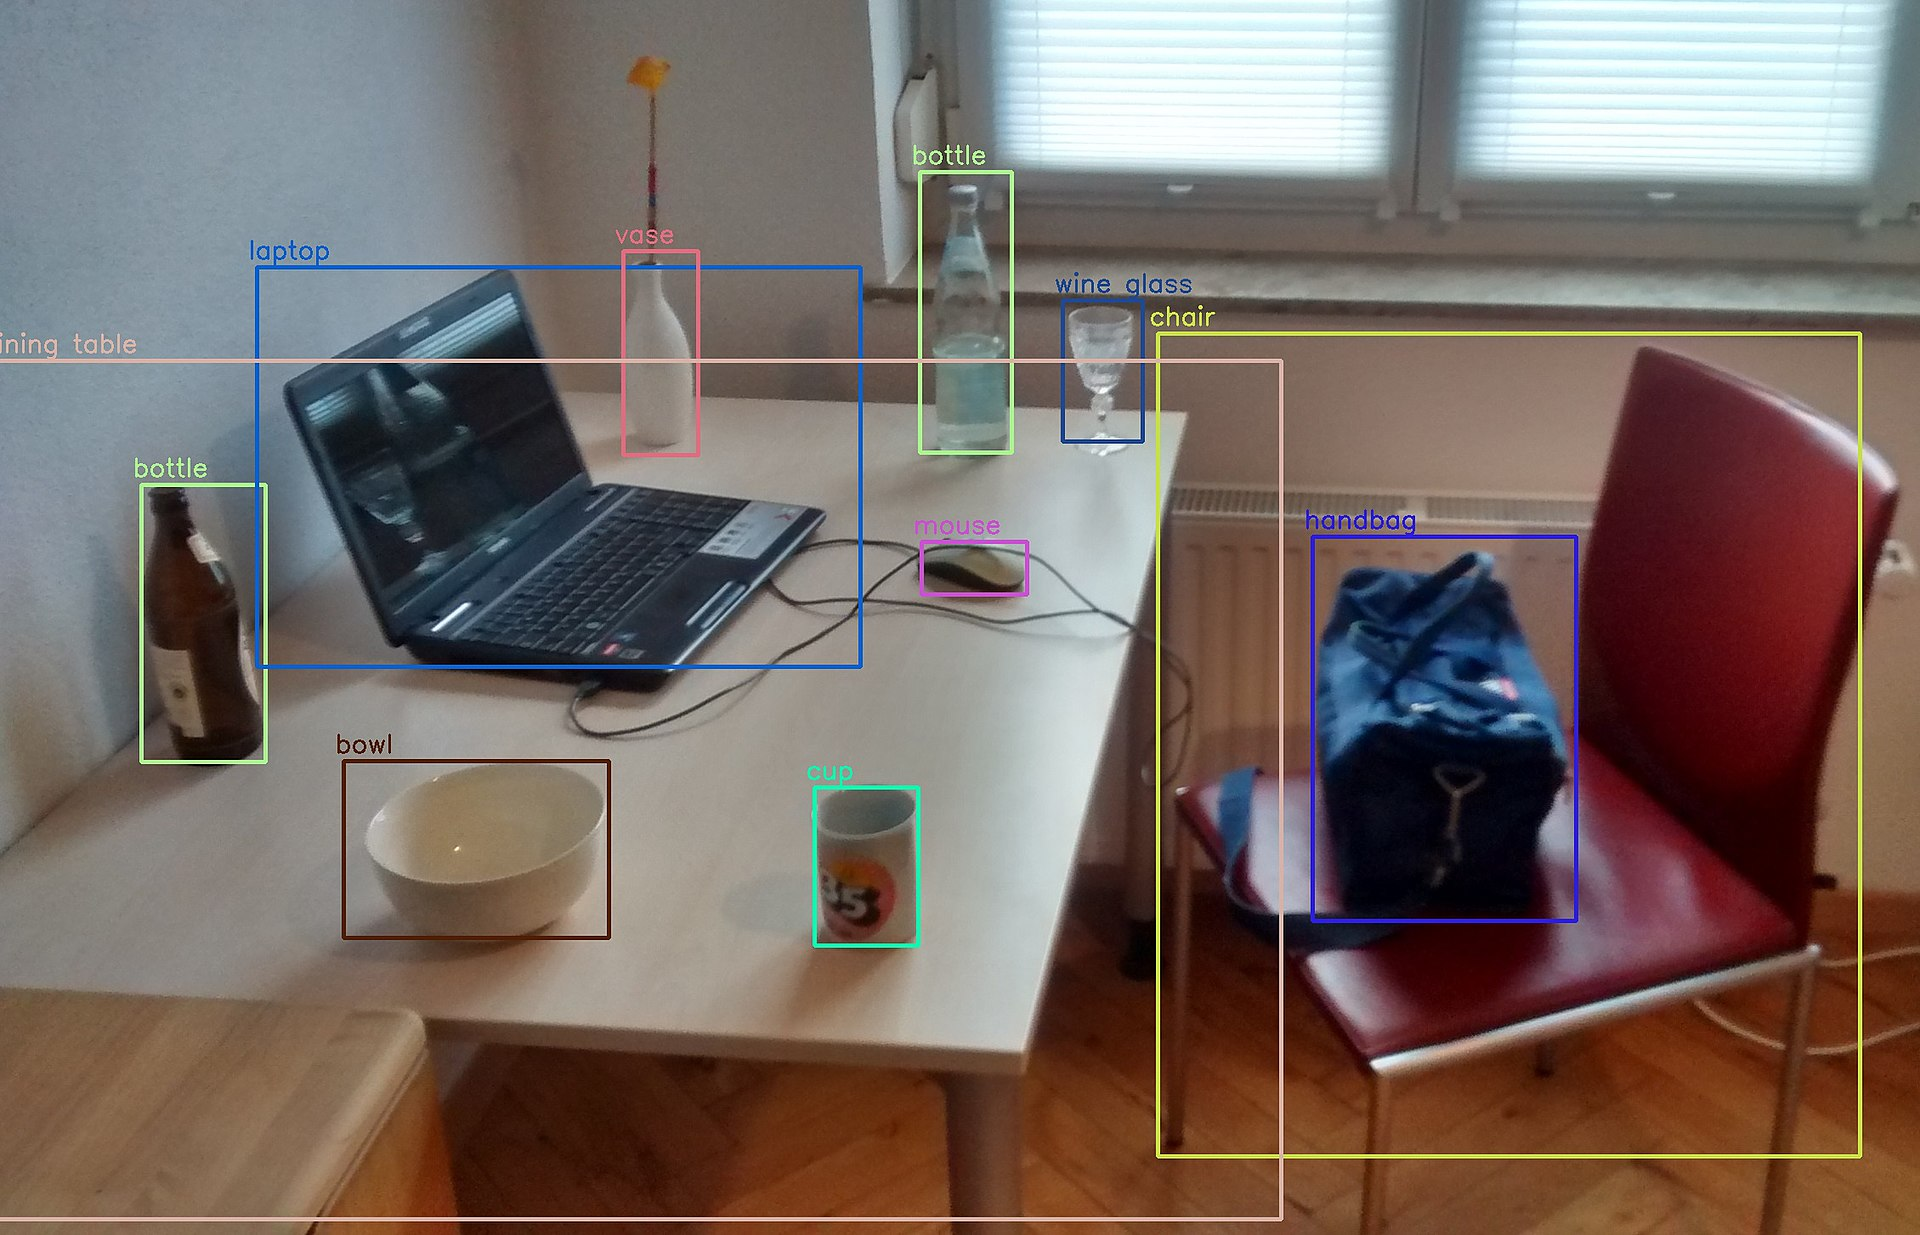
\includegraphics[width=1\textwidth]{images/real_objects.jpg}
            \caption{Image wikipédia qui montre les résultats obtenus d'une détection d'objets à l'aide de l'algorithme YOLOv3 (You Only Look Once) ainsi que le module DNN d'OpenCV. Ce modèle peut détecter jusqu'à 80 objets.}
            \label{}
        \end{figure}
        L'avantage de cette technique c'est qu'elle permet de reconnaître des objets en temps réel dans, par exemple, une vidéo. Dans cette partie, on évoque la manière dont on génère les données qui servent comme entrée pour un modèle pré-entraîné fourni par l'API de détection d'objets de TensorFlow.
        \subsubsection{Une anomalie est un objet}
        Après avoir consulter le fonctionnement basique de l'API de détection d'objets, on a constaté que celle-ci demande un format très particulier (un fichier binaire TFRecord) ainsi qu'une configuration assez compliquée (un fichier .config avec les configurations possibles du modèle). Les anomalies présent dans une image doivent être identifiées et isolées chacune dans sa propre bounding box. L'outil qui permet de faire cette manipulation porte le nom de \textit{LabelImg}. Cet outil permet de générer un fichier csv comportant les colonnes suivantes: \textit{filename} (le nom de fichier d'image où l'anomalie se trouve), \textit{width} (la largeur de l'image), \textit{height} (la hauteur de l'image), \textit{class} (la classe/libellé/étiquette de l'image, \textbf{malfunction} dans notre cas), \textit{xmin} (coordonnée x du 1er point de la bounding box), \textit{ymin} (coordonnée y du 1er point de la bounding box), \textit{xmax} (coordonnée x du 2ème point de la bounding box) et \textit{ymax} (coordonnée y du 2ème point de la bounding box). Cependant, pour générer une énorme base de données d'anomalies isolées, il en faut beaucoup de temps et une main d'œuvre importante. On présente une autre méthode pour résoudre ce problème.
        \begin{figure}[H]
            \centering
            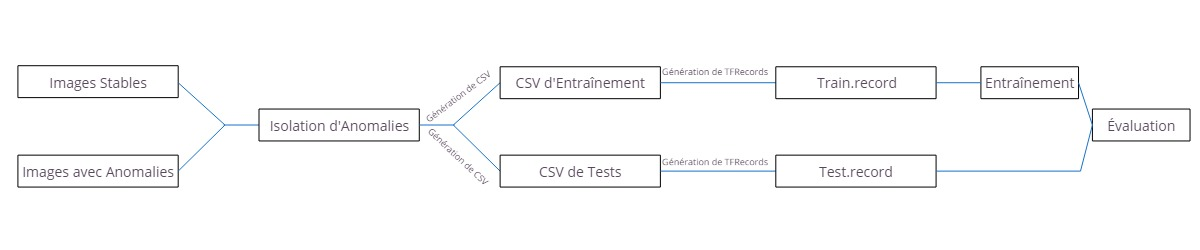
\includegraphics[width=\textwidth]{images/od_datagen.jpg}
            \caption{Pipeline de génération de données pour l'entraînement du modèle de TensorFlow Object Detection API}
            \label{}
        \end{figure}
        \indent Vu qu'on a une version stable d'un système à temps réel ainsi qu'un version avec des anomalies, à l'aide de la librairie de traitement d'images OpenCV, on procède aux manipulations suivantes:
        \newline
        Soit une simulation $S$ d'un système à temps réel commençant à un temps $t$, ayant une durée $d$. On capture la courbe d'état des deux version (stable et avec anomalies) de $t$ à $t+d$ en tant qu'image.
        \newline
        Soit $M_{stable}$ la matrice de pixel de l'image du système stable capturée, et soit $M_{malfunction}$ la matrice de ce même système mais avec une forte présence d'anomalies.
        L'algorithme est le suivant:
        \begin{enumerate}
            \item $M_{diff} = M_{stable} - M_{malfunction}$
            \item On applique 2 fois le filtre \textbf{erode} d'OpenCV (érosion) sur $M_{diff}$ pour se débarrasser des petits clusters de pixels. On a une petite perte d'information sur cette étape qui se compense sur le fait de négliger les anomalies de taille moins importante dû à une erreur de lecture peu fréquente, par exemple.
            \item On applique la fonction \textbf{inRange} d'OpenCV pour obtenir le masque d'image $Mask$ qui extrait les pixels ayant une valeur entre deux gammes de couleurs. Pour notre cas, vu que nos images sont presque similaire, la matrice de pixels $M_{diff}$ admet des couleurs entre le noir et le blanc, le noir étant la couleur de fond et le blanc est le résidu issue de la soustraction. Le masque capture ce résidu.
            \item On applique la fonction \textbf{findContours} d'OpenCV, qui renvoie la liste des contours (bounding box) de chaque cluster de résidu dans $Mask$.
            \item Pour chaque contour trouvé, on extrait le rectangle minimale qui enveloppe ce contour avec la fonction \textbf{boundingRect} d'OpenCV.
            \item Pour chaque bounding box, on écrit la ligne correspondante dans un csv avec les données mentionnées précédemment.
        \end{enumerate}

        \begin{figure}[H]
            \begin{subfigure}{\linewidth}
                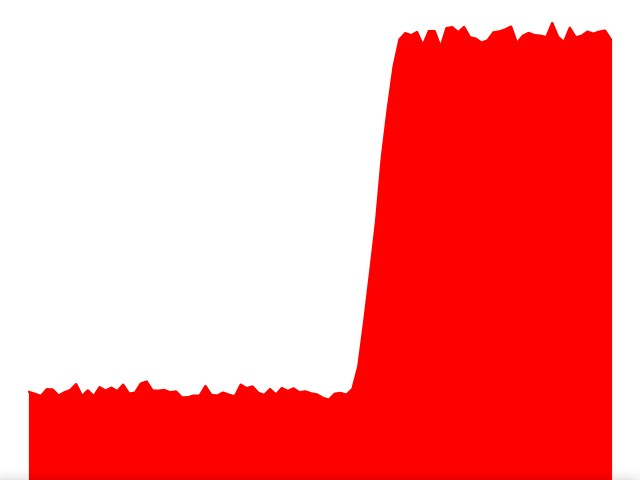
\includegraphics[width=.3\linewidth]{images/od_stable.jpg}\hfill
                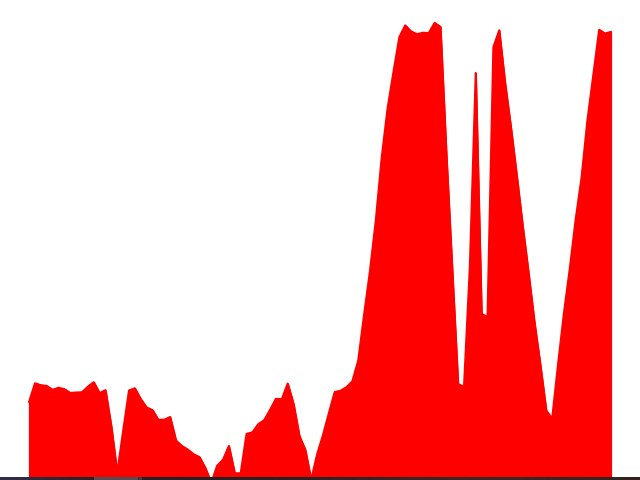
\includegraphics[width=.3\linewidth]{images/od_malfunction.jpg}\hfill
                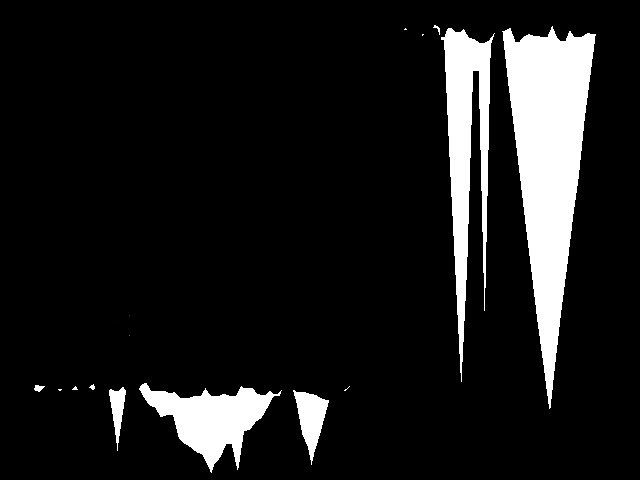
\includegraphics[width=.3\linewidth]{images/od_isolated.jpg}
                \caption{La figure à gauche repésente l'image du système $stable$, au milieu $malfunction$ avec des fortes perturbations, à droite l'image résultante de l'opération de soustraction des matrices de pixels des deux: $M_{diff}$ (1. de l'algorithme ci-dessus)}
            \end{subfigure}\par\medskip
            \begin{subfigure}{\linewidth}
                \hfill
                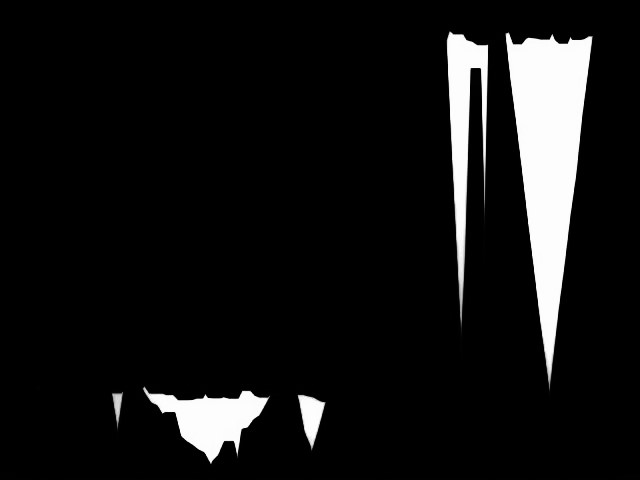
\includegraphics[width=.4\linewidth]{images/od_erosion.jpg}
                \hfill
                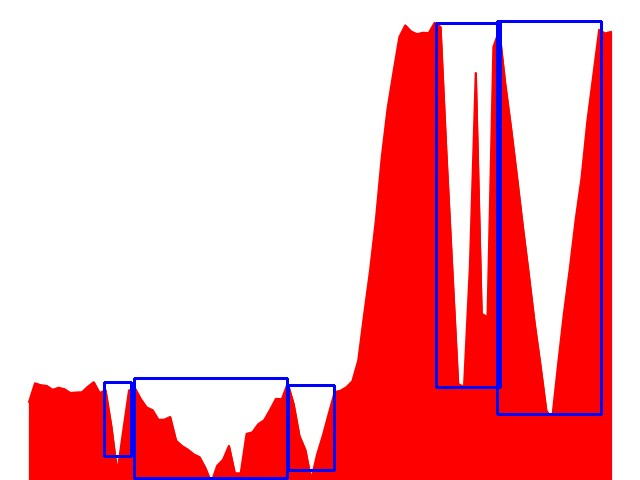
\includegraphics[width=.4\linewidth]{images/od_identified.jpg}
                \hfill
                \caption{La figure à gauche représente l'image issue de la matrice de pixel $M_{diff}$ après l'application du filtre d'érosion, à droite le résultat des opérations 3, 4 et 5 de l'algorithme ci-dessus.}
            \end{subfigure}\par\medskip
        \end{figure}
        \subsubsection{Entraînement du modèle}
        TensorFlow Object Detection API offre plusieurs modèles pré-entraînés. Pour notre entraînement, on a opté pour le modèle \textbf{ssd\_mobilenet\_v1\_coco}\cite{pretrainedmodel} qui utilise MobileNet développé par Google. Ce dernier offre une latence de détection de 30ms et un score mAP (mean Average Precision) de 21. Pour la détection d'objets en général, un compromis entre précision et vitesse est à envisager. Après avoir modifier la configuration de ce modèle pour la prise en compte de nos données (les deux fichiers d'entraînement et de test en format TFRecord), on le lance avec un nombre de batch de $12$ et un nombre maximale d'itérations à la $15 000$ pour ne pas avoir à entraîner le modèle indéfiniment. L'éxecution a été faite avec une machine possédant un processeur Intel i5 avec une fréquance de $2.3GHz$ et une carte graphique NVIDIA GTX960M doté de la technologie CUDA et 8Go de RAM. Sous limite de mémoire, on a réussi à n'avoir que 320 bounding boxes pour l'exécution du modèle, dont 60 sont des données de test/validation et 260 sont utilisés par le modèle pour du fine-tuning d'entraînement. En premier lieu, on a essayé de lancer l'entraînement directement sur le processeur. On constate un écroulement de $12$ secondes entre chaque itération du modèle. Si on le laissait tourner jusqu'à la fin, cela prendra à peu près $67$ heures. On a finalement opté pour un entraînement sur la carte graphique qui, pour chaque itération, prend $0.5$ secondes soit $3$ heures en total. L'API récolte aussi des statistiques concernant le modèle après chaque centaines d'itérations, ce qui consomme à son tour considérablement le temps d'éxecution.
        \newline
        \indent L'entraînement a duré $\sim 11$ heures. Dans la section 5, on discute des résultats qu'on a eu ainsi du potentiel de l'utilisation d'une telle technique pour résoudre le problème de l'entreprise.

    \section{Analyses et Interprétations}
    \subsection{Approche naïve avec CNN}
    Le choix des hyperparamètres du modèle était directement influencé par la limite de ce que nos machines personnelles peuvent gérer. Le modèle qu'on a choisit produit 33 millions de paramètres (poids du réseau de neurones + bias). Mettre une couche de plus avec, disant, 128 filtres, sort l'exception \textit{ResourceExhausted} qui indique que la mémoire ne suffit pas pour entraîner le modèle.
    \newline
    \indent Les résultats qu'on a eu concernant cette approche étaient un peu décevante. Le modèle conçu overfit. Si on considère que les mesures d'accuracy et de loss, il peut sembler que le modèle est plus ou moins bon pour reconnaître les images avec anomalies de ceux sans anomalies. Le point décisif était de voir l'erreur. Ci-dessous les courbes associées pour chaque mesure ainsi que leurs corrélations. La fonction de loss utilisée est \textit{Binary Cross Entropy} : $BCE = -\dfrac{1}{N} \sum\limits_{y \in Y} y \times log(p(y)) + (1-y) \times log(1-p(y))$
    \begin{figure}[H]
        \centering
        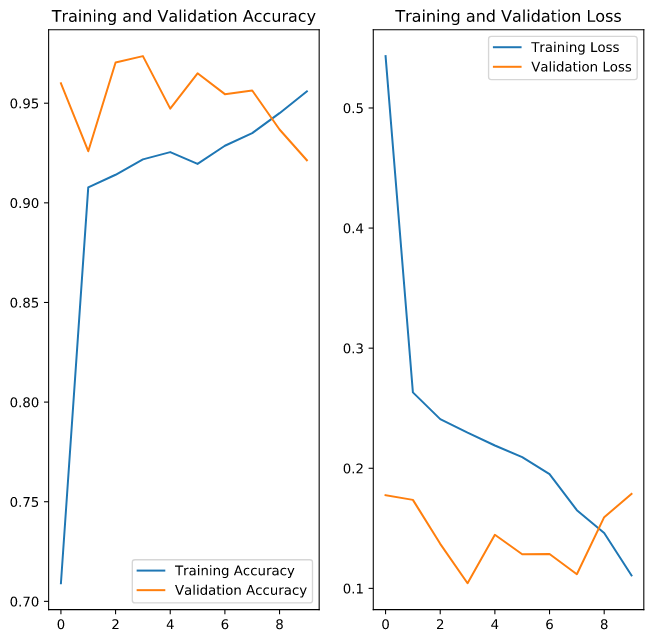
\includegraphics[width=.8\textwidth]{images/cnn_acc_loss.png}
        \caption{La figure de gauche représente l'accuracy par rapport à nombre d'epochs, celle de droite représente le loss. On observe bien une accuracy entre 0.9 et 0.97 pour les ensembles d'images d'entraînement et de validation ainsi qu'une pente de perte descendante et proche de 0 pour les deux aussi.}
        \label{}
    \end{figure}
    La fonction d'erreur utilisé est $MSE = \dfrac{1}{n}\sum\limits_{y \in Y} (y - \hat{y})^2$ avec $\hat{y}=\dfrac{1}{n}\sum\limits_{y \in Y} y$
    \begin{figure}[H]
        \centering
        \begin{subfigure}{\linewidth}
            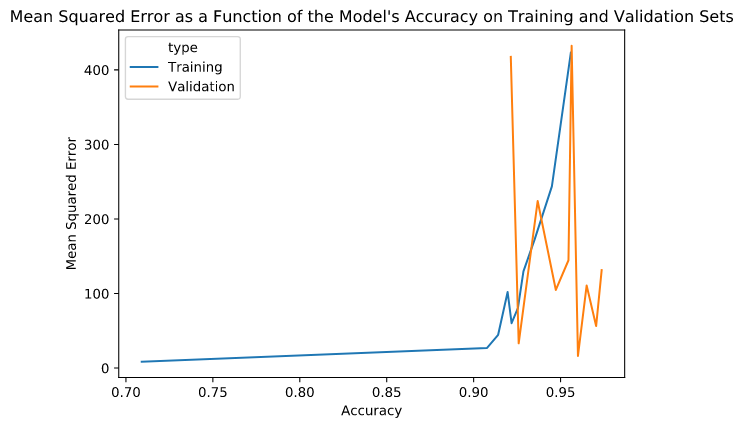
\includegraphics[width=.49\textwidth]{images/cnn_mse_acc.png}
            \hfill
            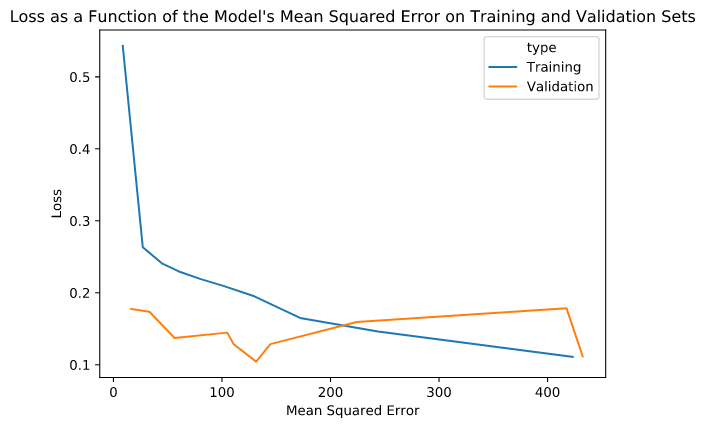
\includegraphics[width=.47\textwidth]{images/cnn_loss_mse.png}
        \end{subfigure}
        \caption{La figure à gauche resprésente l'erreur en fonction de l'accuracy et celle de gauche la perte par rapport à l'erreur. On constate que l'erreur varie d'une manière très irrégulière pour l'ensemble de validation et de manière exponentielle dans l'ensemble d'entraînement pour la figure gauche, de plus, dans celle de droite on observe que quand la perte est converge vers 0, l'erreur augmente considérablement.}
        \label{}
    \end{figure}
    L'erreur nous indique clairement que les métriques d'accuracy et de loss ne sont pas indiquant de la performance du modèle. Avec un taux d'erreur important, on peut conclure que le modèle overfit et qu'il n'est apte qu'à classifier les instances qu'il connaît déjà d'où les fluctuations de l'erreur pour l'ensemble de validation.
    
    \subsection{Extraction des features avec TSFresh}

      Nous avons constaté lorsque nous avons extrait les features avec TSFresh que la majorité des features les plus pertinentes étaient des coefficient de séries de Fourier.
        Nous pensons que cela est dû au fait que nos séries se généralisent très bien en des additions de sinuisoïdales. En effet, une série sans malfonctions est en réalité une répétition d'états actifs et au repos ayant une amplitude à peu près stable (en fonction du bruit); elle ressemble à un signal carré (imparfait, puisque les transitions entre les états ne sont pas instantanées).
        
        \begin{figure}[H]
            \centering
            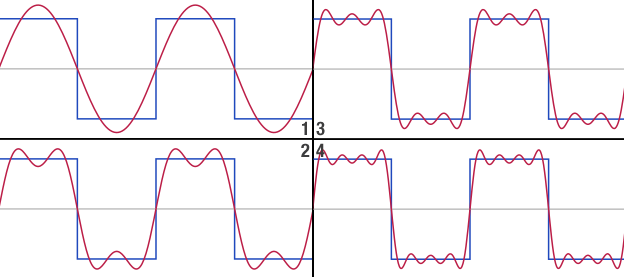
\includegraphics[width=0.3\textwidth]{images/signal_carre.png}
            \caption{Image de Wikipédia illustrant les quatre premières sommes partielles d'une série de Fourier pour approximer un signal carré.}
            \label{}
        \end{figure}
        
        En revanche, lorsque des malfonctions sont présentes dans une série, elles génèrent de plus nombreux pics haut et bas d'amplitudes à intervalles irréguliers. Ces nombreux pics empêchent d'obtenir une image relativement proche de notre courbe uniquement avec les coefficients de basse fréquence de la série de Fourier. C'est donc un indicateur simple permettant de déterminer si une série temporelle représentant la pression des senseurs présente des malfonctions ou non.
        
        Il faut cependant considérer que cela est vrai à condition que l'hypothèse que nosu avons fait dans notre simulateur en fonction des données réelles auxquelles nous avons rapidement eu accès se vérifie: Les périodes des états actifs et au repos sont relativement stables. En effet, il est beaucoup plus difficile d'approximer un signal carré irrégulier avec seulement quelques coefficients d'une série de Fourier. De plus, il devient alors difficile de dissocier des pics dûs à des malfonctions de simples changement d'états anticipés.
        
    Un autre aspect est que bien que nous avons trié les features en fonction de leur pouvoir prédictif, ces tests se font de façon individuelle sur chacune des features. Hors on ne peut pas exclure que certaines features soient plus ou moins efficaces dans certaines combinaisons. Ainsi, pour être sûr d'avoir l'ensemble réduit de N features le plus efficace, il faudrait tester toutes les permutations possibles et non seulement les N premiers, ce que nous n'avons pas fait pour des raisons de temps de calcul.
    
    Enfin, bien nous ayons tenté de limiter l'overfit autant que possible, en l'absence d'un jeu de données réel conséquent fourni par la société, nous ne pouvons être confiants de nos résultats uniquement sur les séries temporelles générées par notre simulateur.
        
        
    \subsection{Détection d'anomalies en tant qu'objets}
    Pour cette approche, on obtient des résultats intéressants. Le modèle reconnaît et isole bien les anomalies avec une certaine probabilité.
    \begin{figure}[H]
        \centering
        \begin{subfigure}{\linewidth}
            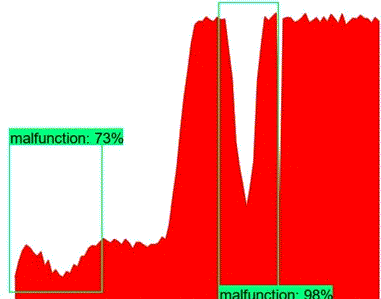
\includegraphics[width=.5\textwidth]{images/od_1.png}
            \hfill
            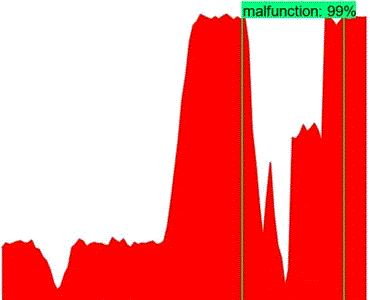
\includegraphics[width=.5\textwidth]{images/od_2.png}
        \end{subfigure}
    \end{figure}
    \begin{figure}[H]
        \centering
        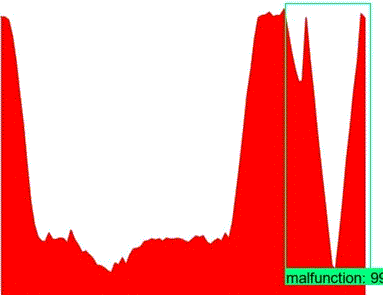
\includegraphics[width=.5\textwidth]{images/od_3.png}
        \caption{La détection d'anomalies sur des images différentes de ceux de l'ensemble d'entraînement semble correcte mais pas parfaite.}
        \label{}
    \end{figure}
    À l'aide de l'application de surveillance de modèles TensorBoard, on peut extraire quelques métriques en liaison avec l'entraînement en temps réel. Cependant, l'application n'expose que des mesures de pertes et d'autres métriques qui ne sont pas documentées. Pour les mesures de perte, on a les résultats suivant:
    \begin{figure}[H]
        \centering
        \begin{subfigure}{\linewidth}
            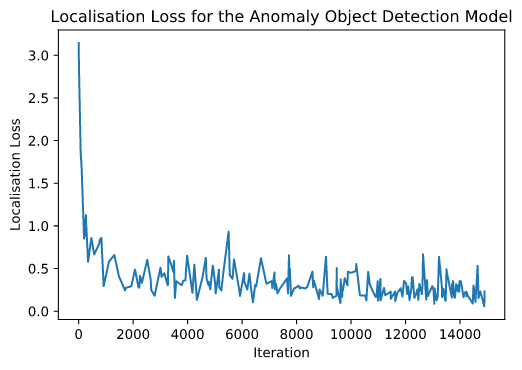
\includegraphics[width=.5\textwidth]{images/od_loc_loss.png}
            \hfill
            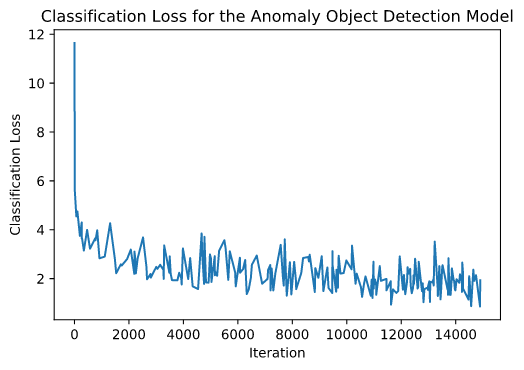
\includegraphics[width=.5\textwidth]{images/od_cla_loss.png}
        \end{subfigure}
        \caption{À gauche, la perte liée à la prédiction des coordonnées des bounding boxes qui entourent les anomalies en fonction du nombre d'itérations écroulé. À droite, celle lié aux prédiction de classification; dire que la partie de l'image entouré présente bien une anomalie ou pas.}
    \end{figure}
    Pour les deux courbes, on observe bien une pente de perte descendante. Celle de localisation est plus ou moins proche de 0, mais celle de classification est entre 1 et 2 à $15000^{\text{ème}}$ itération. Selon la documentation sur la configuration du modèle, l'API dit qu'un nombre d'itérations de $200000$ est recommandé afin d'obtenir une perte entre 0 et 1.
    \newline
    \indent On n'a pas de résultats conclusifs sur la précision et la fidélité du modèle. La perte nous nous donnes pas assez d'informations comme on a pu s'aperçevoir dans le modèle CNN naïve. De plus, ni le nombre d'itérations, ni le nombre de données ne sont suffisant pour prendre en considération toutes les formes possibles d'une anomalie. L'avantage de cette approche sont quand même à prendre en considération. L'API de Détection d'Objets de TensorFlow n'est pas assez documenté pour faire des expériences plus sophistiquées avec des résultats pertinants et analysables. La migration de la version 1 à la version 2 a donné naissance à plusieurs bugs ainsi que plusieurs modules obsolètes qui demandent des contournements pour qu'ils fonctionnent à nouveau. Il sera peut-être plus judicieux de faire jouer la concurrence et de regarder les résultats qu'on obtient avec une librairie de Deep Learning comme PyTorch qui est plutôt plus stable et de plus en plus adoptée.
    \newline
    \indent Néanmoins, une détection d'anomalies en temps réel est très utile au sein d'un système, aussi, à temps réel. L'entreprise peut opté pour cette approche dans le cadre où celle-ci est prouvé être fonctionnel avec des analyses et des métriques qui le montre et que nous avons pas eu les ressources pour le faire.
    \section{Conclusion}

\renewcommand\refname{7\indent Références}
\begin{thebibliography}{1}
\bibitem{odwikipedia} \href{https://en.wikipedia.org/wiki/Object\_detection}{Wikipedia, Object Detection}
\bibitem{pretrainedmodel} \href{https://github.com/tensorflow/models/blob/master/research/object_detection/g3doc/detection_model_zoo.md#coco-trained-models}{TensorFlow, \textit{models} repository, Tensorflow detection model zoo.}
\bibitem{tsfreshfeatures} \href{https://tsfresh.readthedocs.io/en/latest/text/list_of_features.html}{Liste des features calculées par TSFresh, TSFresh documentation}
\end{thebibliography}

\end{document}